\documentclass[oneside,10pt]{scrartcl}
\usepackage{graphicx}
\usepackage{float}
\usepackage{geometry}
\usepackage{multicol}
\usepackage{hyperref}
\usepackage{tcolorbox}

\graphicspath{{./images/}}
\newgeometry{left=20mm,right=20mm,top=20mm,bottom=20mm}
%\pagenumbering{gobble}
\setlength\columnsep{20pt}
\setlength{\parindent}{0cm}

\title{Mathmatics for Machine Learning - Cheatsheet}
\author{}
\date{}

\begin{document}
\pagenumbering{roman}
\maketitle
\tableofcontents
\newpage
\pagenumbering{arabic}
\footnotesize

\begin{multicols*}{2}
%%%%%%%%%%%%%%%%%%%%%%%%%%%%%%%%%%%%%%%%%%%%%%%%%%%%%%%%%%%%%%%%%%%%%%%%%%%%%
%%%%%%%%%%%%%%%%%%%%%%%%%%%%%%%%%% General %%%%%%%%%%%%%%%%%%%%%%%%%%%%%%%%%%
%%%%%%%%%%%%%%%%%%%%%%%%%%%%%%%%%%%%%%%%%%%%%%%%%%%%%%%%%%%%%%%%%%%%%%%%%%%%%
\section{General}

\begin{figure}[H]
\centering
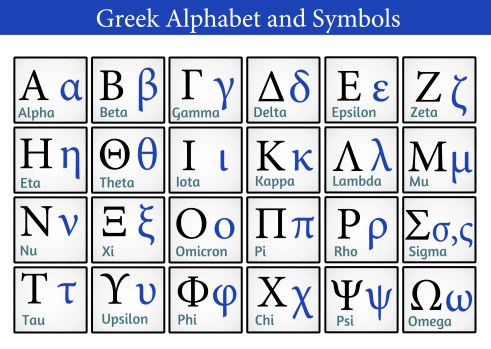
\includegraphics[width=\linewidth]{greek-alphabet}
\caption{\url{https://www.greekboston.com/wp-content/uploads/2016/02/greek-alphabet.jpg}} \label{fig:greek_alphabet}
\end{figure}

\newpage

%%%%%%%%%%%%%%%%%%%%%%%%%%%%%%%%%%%%%%%%%%%%%%%%%%%%%%%%%%%%%%%%%%%%%%%%%%%%%
%%%%%%%%%%%%%%%%%%%%%%%%%%%%%%%%%% Linear Algebra %%%%%%%%%%%%%%%%%%%%%%%%%%%
%%%%%%%%%%%%%%%%%%%%%%%%%%%%%%%%%%%%%%%%%%%%%%%%%%%%%%%%%%%%%%%%%%%%%%%%%%%%%
\section{Linear Algebra}

\subsection{Matrices}
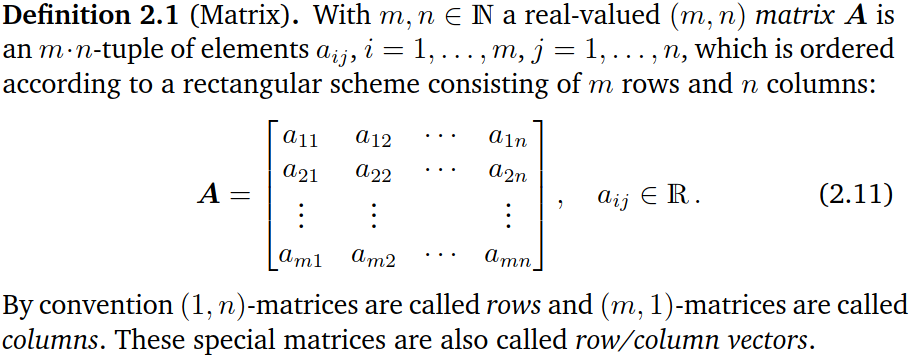
\includegraphics[width=\linewidth]{2.2}

\subsubsection*{Operation Properties}
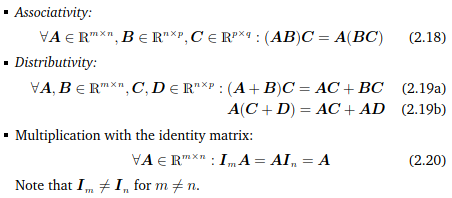
\includegraphics[width=\linewidth]{2.2_1}

\subsubsection*{Inverse}
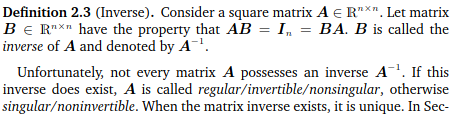
\includegraphics[width=\linewidth]{2.2_2}

\subsubsection*{Transpose, Symmetry and other Properties}
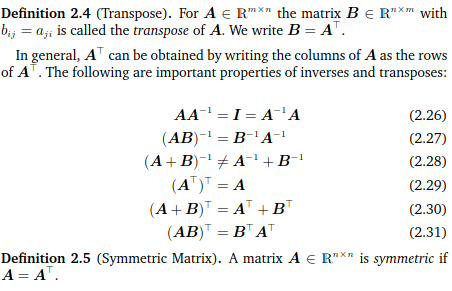
\includegraphics[width=\linewidth]{2.2_3}


\subsection{Solving System of Linear Equations}
\subsubsection*{Row-Echelon Form}
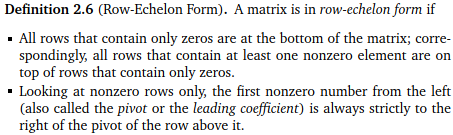
\includegraphics[width=\linewidth]{2.3}

\subsubsection*{Reduced-Row-Echelon Form}
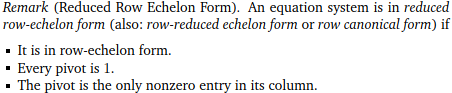
\includegraphics[width=\linewidth]{2.3_1}
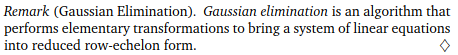
\includegraphics[width=\linewidth]{2.3_2}
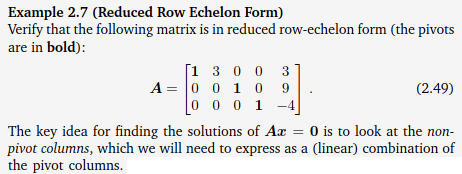
\includegraphics[width=\linewidth]{2.3_5}

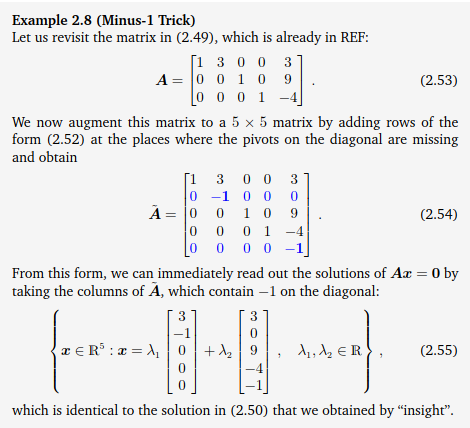
\includegraphics[width=\linewidth]{2.3_3}
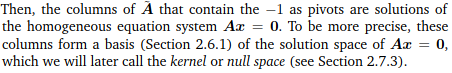
\includegraphics[width=\linewidth]{2.3_6}

\subsubsection*{Calculation of Matrix Inverse}
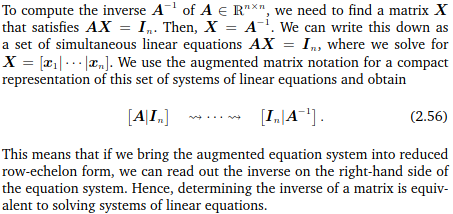
\includegraphics[width=\linewidth]{2.3_4}


\subsection{Vector Spaces}
\subsubsection*{Groups}
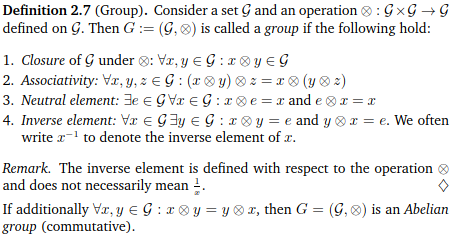
\includegraphics[width=\linewidth]{2.4}
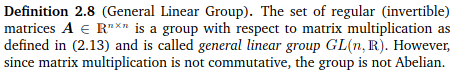
\includegraphics[width=\linewidth]{2.4_1}

\subsubsection*{Vector Spaces}
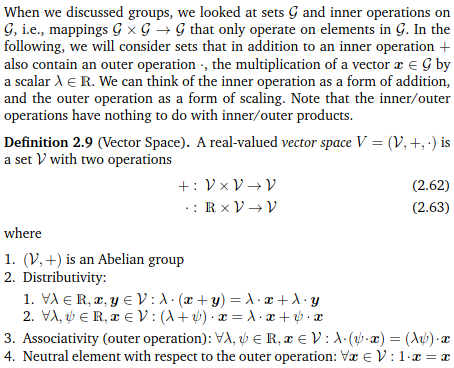
\includegraphics[width=\linewidth]{2.4_2}

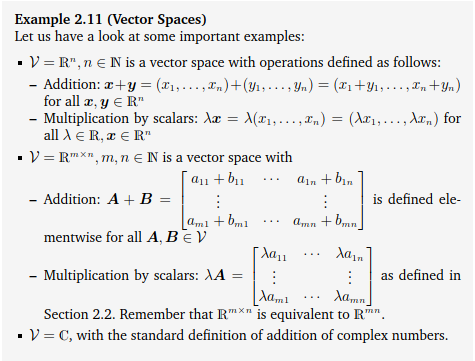
\includegraphics[width=\linewidth]{2.4_3}

\subsubsection*{Vector Subspaces}
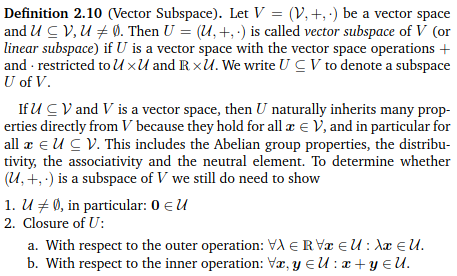
\includegraphics[width=\linewidth]{2.4_4}

\subsection{Linear Independence}
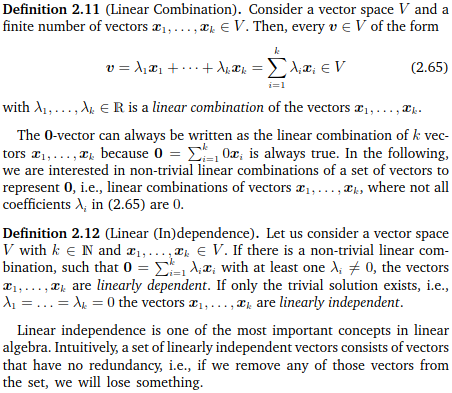
\includegraphics[width=\linewidth]{2.5}

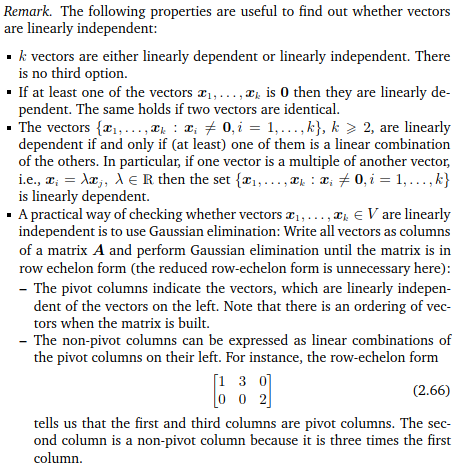
\includegraphics[width=\linewidth]{2.5_1}

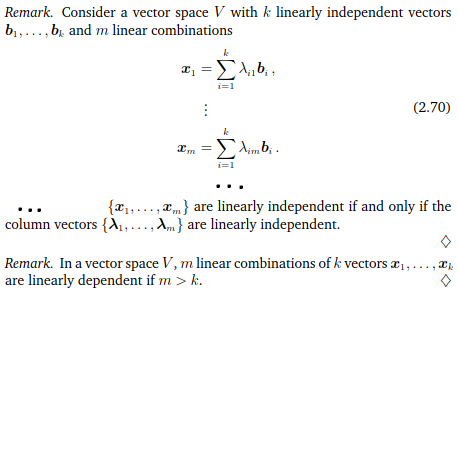
\includegraphics[width=\linewidth]{2.5_2}


\subsection{Basis and Rank}

\subsubsection*{Generating Set and Basis}
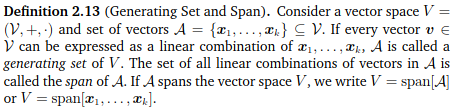
\includegraphics[width=\linewidth]{2.6}

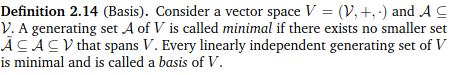
\includegraphics[width=\linewidth]{2.6_1}

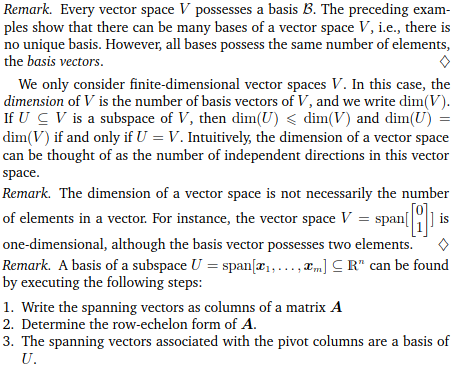
\includegraphics[width=\linewidth]{2.6_2}

\subsubsection*{Rank}
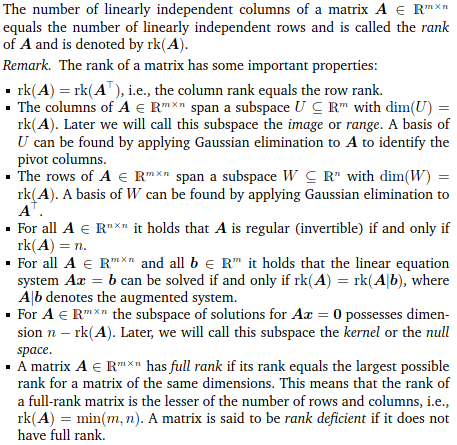
\includegraphics[width=\linewidth]{2.6_3}


\subsection{Linear Mappings}
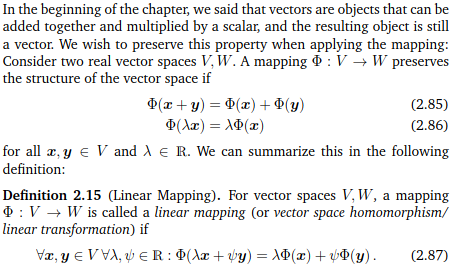
\includegraphics[width=\linewidth]{2.7}

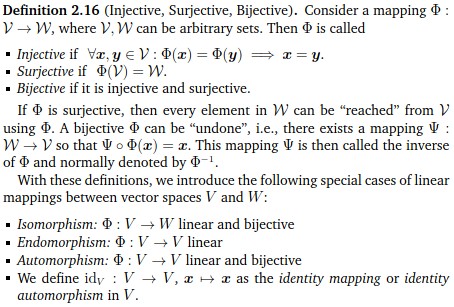
\includegraphics[width=\linewidth]{2.7_1}

\begin{tcolorbox}
\textbf{Injective} means we won't have two or more "A"s pointing to the same "B".

\textbf{Surjective} means that every "B" has at least one matching "A" (maybe more than one). 

\textbf{Bijective} means both injective and surjective together (perfect "one-to-one correspondence" between the members of the sets).

{\tiny \url{https://www.mathsisfun.com/sets/injective-surjective-bijective.html}}
\end{tcolorbox}

\begin{tcolorbox}
\textbf{Homomorphism}: structure-preserving map between two algebraic structures of the same type (such as two groups, two rings, or two vector spaces)

\textbf{Isomorphism}: mapping between two structures of the same type that can be reversed by an inverse mapping. Two mathematical structures are isomorphic if an isomorphism exists between them.

\textbf{Endomorphism}: a morphism from a mathematical object to itself. An endomorphism that is also an isomorphism is an \textbf{automorphism}.

{\tiny Wikipedia}
\end{tcolorbox}

\end{multicols*}
\end{document}